\documentclass[10pt,xcolor={table,dvipsnames},t]{beamer}
\usetheme{UCBerkeley}
\usepackage{ctex}
\bibliography{ref}

\title{Turbulence phenomenology}
\subtitle{The Gioia way.}
\author{刘宁}
\institute{浙江大学}
\date{\today}

\begin{document}

\begin{frame}
  \titlepage
\end{frame}

\begin{frame}{Velocity component at $s$ scale}
    \begin{align*}
        u_s^2 = \int_0^s E(\sigma) \sigma^{-2} d\sigma = \int_{1 / s}^{\infty} E(k) dk
    .\end{align*}
    with $E(\sigma) \sim \varepsilon^{2 / 3} \sigma^{5 / 3} \mathbf{c_d} \left( \eta / \sigma \right) \mathbf{c_e} \left( R / \sigma \right)$ and $E(k) \sim \varepsilon^{2 / 3} k^{-5 / 3} \mathbf{c_d} (\eta k) \mathbf{c_e} \left( Rk \right) $ \footnote{Note: \citet{gioiaFriction2006}中使用$\mathbf{c_e} \left( \sigma / R \right) $ 形式,注意到$R / \sigma = Rk$,为了$\mathbf{c_e} $ 的统一形式将其定义为$\mathbf{c_e} \left( R / \sigma \right) $.}.

    \begin{align*}
        \begin{cases}
            \mathbf{c_d}\left( x \right)  = \exp\left( -\beta_d x \right) \\
            \mathbf{c_e} \left( x \right) = \left( 1+\beta_e x^{-2} \right) ^{-17 / 6} 
        \end{cases}
    .\end{align*}

    $\mathbf{c_d}$ 形式来自\citet{gioiaFriction2006},$\mathbf{c_e}$ 取自von K\'arm\'an. 在惯性区$\eta \ll s \ll R$ ,两个修正项均为$1$.
    
\end{frame}

\begin{frame}{The uniform form of velocity $u_s$}
    Let $\xi = sk = s / \sigma$, rewrite $u_S$ in a uniform form:
    \begin{align*}
        u_s \sim \left( \varepsilon s \right) ^{1 / 3} \left[ \int_1^{\infty} \xi^{-5 / 3} \mathbf{c_d}\left( \frac{\eta}{s} \xi \right) \mathbf{c_e} \left( \frac{R}{s} \xi \right) d\xi \right]^{1 / 2}  \triangleq \left( \varepsilon s \right) ^{1 / 3} \sqrt{\mathcal{I} } 
    .\end{align*}
    \begin{block}{Takeaway msg}
        \begin{itemize}
            \item $u_s \sim \left( \varepsilon s \right) ^{1 / 3} $ in inertial range ($\eta \ll s \ll R$).
            \item 提取涡体(尺度为$s$)特征速度$u_s$ 的问题转化为修正函数$\mathcal{I}$ 的讨论,$\mathcal{I}\left( \eta / s, R / s \right)  \triangleq \int_1^{\infty} \xi^{-5 / 3} \mathbf{c_d}\left( \frac{\eta}{s} \xi \right) \mathbf{c_e} \left( \frac{R}{s} \xi \right) d\xi$.
        \end{itemize}
    \end{block}
\end{frame}

\begin{frame}{The phenomenology big picture}
    \begin{itemize}
        \item Energy cascade
            \begin{align*}
                u_s^3 / s \sim u_R^3 / R
            .\end{align*}
            \begin{itemize}
                \item With $\varepsilon \sim u_R^3 / R$, $\eta = \left( \nu^3 / \varepsilon \right)^{1 / 4}\sim R\cdot Re^{-\frac{3}{4}} $.
            \end{itemize}
    \end{itemize}
\end{frame}

\begin{frame}{The Gioia way: Local shear stress model}
    Eddies $\left( u_s, s \right) $ that straddle wetted surface $W_y\implies $ shear stress $\tau$,
    \begin{itemize}
        \item $v_t$ 代表涡体能够传递的动量大小,取决于湿面积两侧的动量差($\propto \frac{\partial u}{\partial y}\cdot s $)
        \item $v_n$ 代表涡体传递动量的速率,取决于涡体的特征速度($\sim u_s$)
    \end{itemize}
    \begin{columns}
        \begin{column}{0.5\textwidth}
            \begin{align*}
                \tau \sim \rho v_t v_n
            .\end{align*}
        \end{column}
        \begin{column}{0.5\textwidth}
            \begin{figure}[htpb]
                \centering
                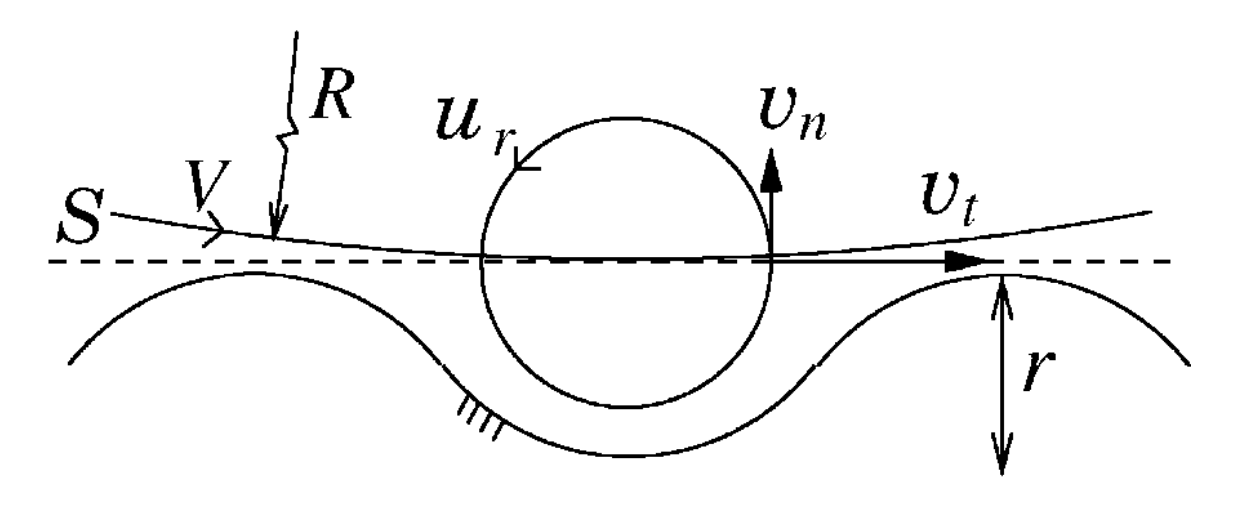
\includegraphics[width=0.5\textwidth]{./figures/eddies.png}
                % \caption{Schematic of eddy phenomenology \cite{gioiaprl2001}.}
                \label{fig:-figures-eddies-png}
            \end{figure}
        \end{column}
    \end{columns}
    \begin{itemize}
        \item Local wall shear stress model \cite{gioiaFriction2006}: $v_t \sim V$, $v_n\sim u_{r+a\eta}$
        \item Local water column shear stress model \cite{gioiaMVP2010}: $v_t\sim u(y+s) - u(y-s)\approx 2s u'(y) \sim 2y\cdot u'(y)$, $v_n \sim u_y$
    \end{itemize}
    \begin{figure}[!htb]
        \centering
        \begin{minipage}{.5\textwidth}
            \centering
            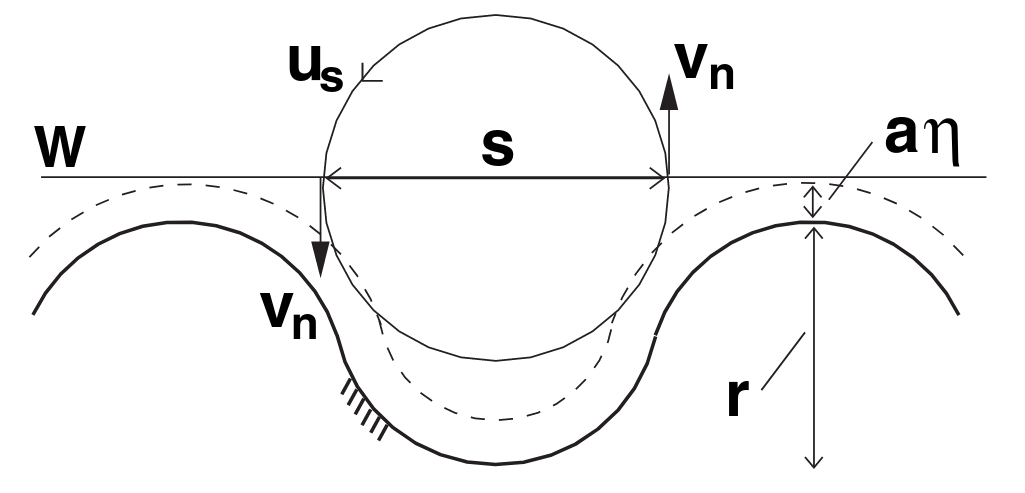
\includegraphics[width=0.6\textwidth]{./figures/wall-shear.png}
            \label{fig:wall-shear}
        \end{minipage}%
        \begin{minipage}{0.5\textwidth}
            \centering
            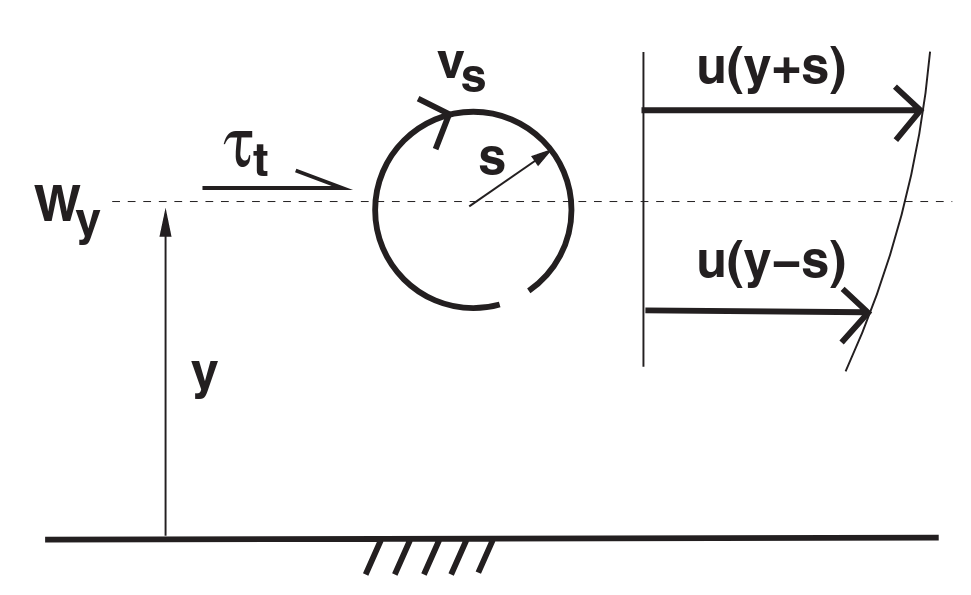
\includegraphics[width=0.6\textwidth]{./figures/column-shear.png}
            \label{fig:column-shear}
        \end{minipage}
    \end{figure}
\end{frame}

\begin{frame}{Unify the local shear stress model}
    \begin{figure}[htpb]
        \centering
        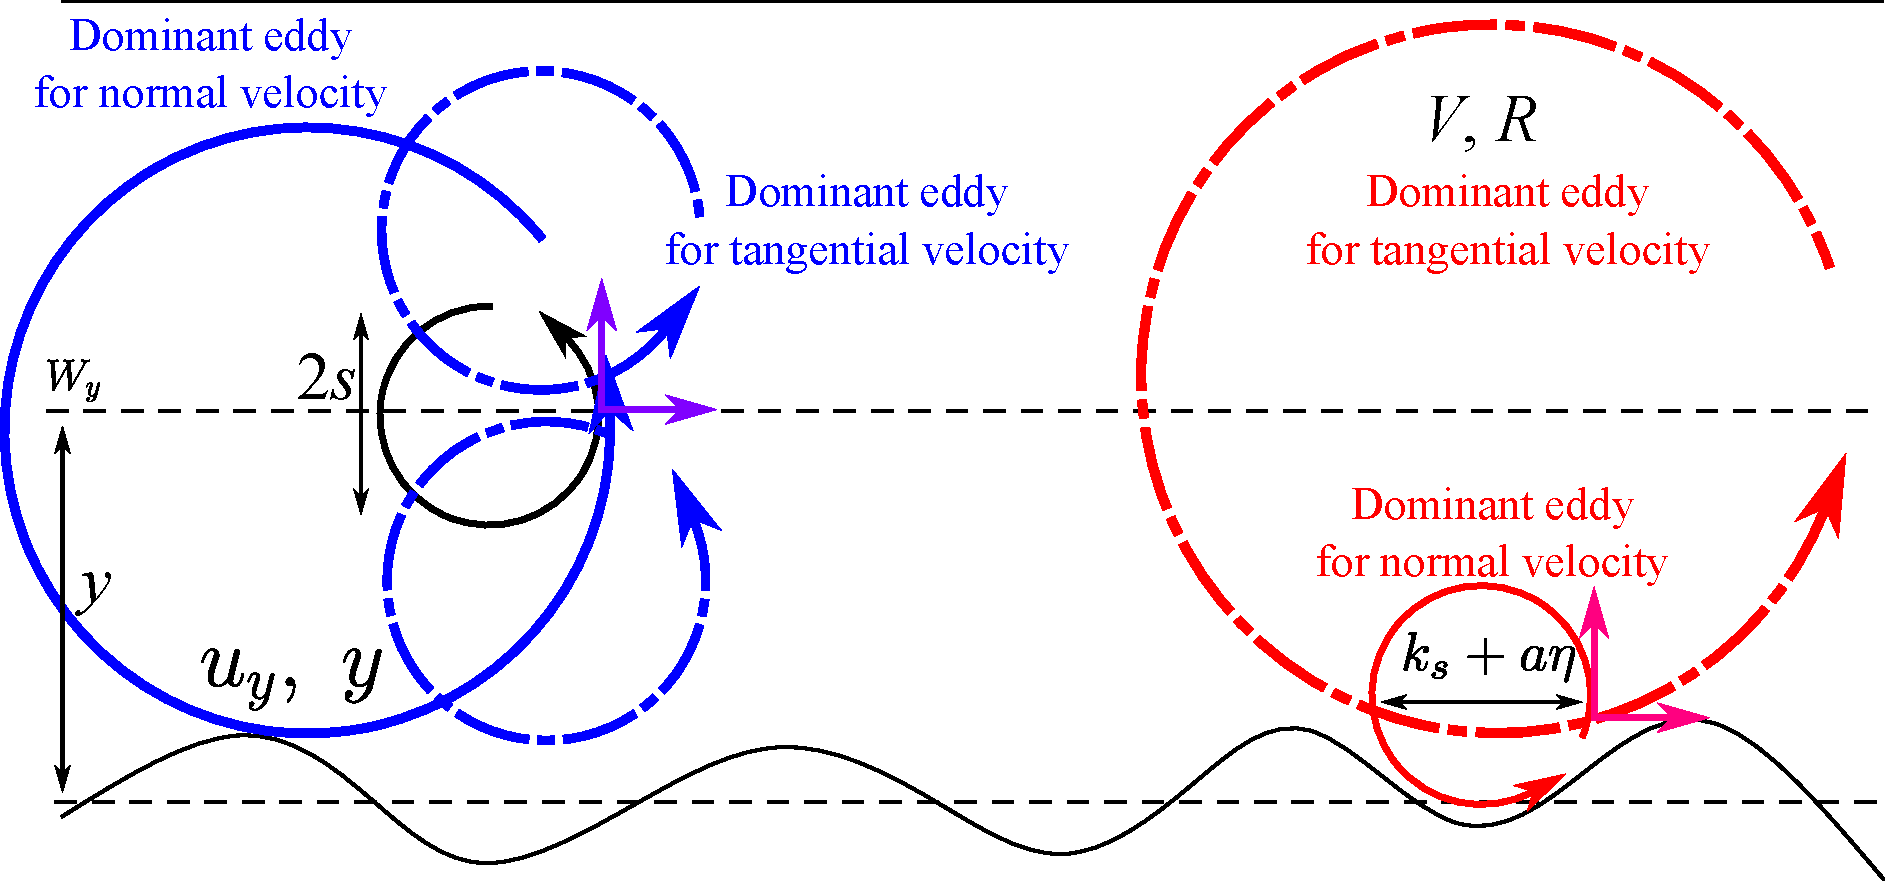
\includegraphics[width=0.8\textwidth]{./figures/unify-gioia-model.pdf}
        \caption{The unified picture of the Gioia model.}
        \label{fig:-figures-unify-gioia-model-pdf}
    \end{figure}
\end{frame}

\begin{frame}{Unify the local shear stress model}
    \begin{itemize}
        \item $v_n$ :近床面位置,特征涡体由粗糙高度$k_s$ 和黏性底层$a\eta$ 共同控制 $s = k_s + a\eta$;外区部分的特征涡体完全由床面高度$y$ 控制\footnote{Townsend 附着涡模型存在类似的特征尺度正比于床面距离的涡体。或许可视作仅考虑外区涡体的特例。}
        \item $v_t$ :Gioia的贡献。
    \end{itemize}
\end{frame}

\begin{frame}[allowframebreaks]
  \frametitle{参考文献}
  \printbibliography[heading=bibliography,title=参考文献]
  % \bibliographystyle{plain} % We choose the "plain" reference style
  % \bibliography{ref} % Entries are in the refs.bib file
\end{frame}

\end{document}
